\documentclass{article}
\usepackage{tikz}
\usetikzlibrary{arrows.meta}
% 箭头符号
\begin{document}
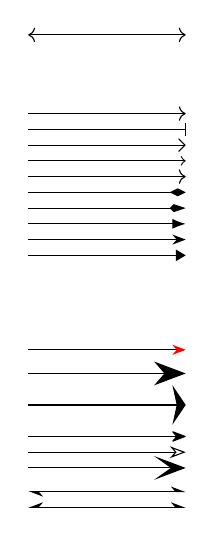
\begin{tikzpicture}
    % 在路径的起始或结束位置使用箭头,需要使用arrows.meta库,参考section 16
    % 使用箭头的格式: arrows=<start_arrow>-<end_arrow>,省略start_arrow或end_arrow时,不显示该箭头
    \draw[arrows=<->] (0,0) -- (2,0);

    % 箭头类型
    \begin{scope}[yshift=-1cm]
	\draw[arrows=->] (0,0) -- (2,0);
	\draw[yshift=-2mm,arrows=-Bar] (0,0) -- (2,0);
	\draw[yshift=-4mm,arrows=-Straight Barb] (0,0) -- (2,0);
	\draw[yshift=-6mm,arrows=-Classical TikZ Rightarrow] (0,0) -- (2,0);
	\draw[yshift=-8mm,arrows=-Computer Modern Rightarrow] (0,0) -- (2,0);
	\draw[yshift=-10mm,arrows=-Diamond] (0,0) -- (2,0);
	\draw[yshift=-12mm,arrows=-Kite] (0,0) -- (2,0);
	\draw[yshift=-14mm,arrows=-Latex] (0,0) -- (2,0);
	\draw[yshift=-16mm,arrows=-Stealth] (0,0) -- (2,0);
	\draw[yshift=-18mm,arrows=-Triangle] (0,0) -- (2,0);
    \end{scope}

    % 设置箭头属性{<arrow>[<attributes>]}. 属性列表:
    % 1.color - 箭头颜色
    % 2.fill - 箭头填充颜色
    % 3.length - 箭头的水平长度
    % 4.width - 箭头的垂直宽度
    % 5.round - 拐角处圆滑过渡
    % 6.sharp - 拐角处尖锐
    % 7.line width - 绘制箭头画笔的宽度
    % 8.open - 箭头空心,类似于fill=none
    % 9.inset - 箭头尾部垂直中点, 向内部凹进去的距离(只对Stealth箭头有效)
    % 10.angle - 格式为<angle>:<dimension>, 箭头头部的角度和头部斜边长度
    % 11.scale - 箭头伸缩系数
    % 12.scale length/scale width - 箭头长度或宽度伸缩系数
    % 13.slant - 箭头倾斜系数
    % 14.reversed - 箭头本身进行翻转
    % 15.harpoon - 只保留沿着箭头方向的左侧
    % 16.swap - 对箭头进行镜像,配合harpoon使用,只保留沿着箭头方向的右侧
    % 17.left/right - left类似于harpoon,right类似于harpoon和swap组合
    \begin{scope}[yshift=-4cm]
	\draw[arrows=-{Stealth[color=red]}] (0,0) -- (2,0);
	\draw[yshift=-3mm,arrows=-{Stealth[length=4mm]}] (0,0) -- (2,0);
	\draw[yshift=-7mm,arrows=-{Stealth[width=5mm]}] (0,0) -- (2,0);
	\draw[yshift=-11mm,arrows=-{Stealth[length=2mm,round]}] (0,0) -- (2,0);
	\draw[yshift=-13mm,arrows=-{Stealth[length=2mm,open]}] (0,0) -- (2,0);
	\draw[yshift=-15mm,arrows=-{Stealth[length=4mm,inset=6pt]}] (0,0) -- (2,0);
	\draw[yshift=-18mm,arrows={Stealth[harpoon]}-{Stealth[harpoon]}] (0,0) -- (2,0);
	\draw[yshift=-20mm,arrows={Stealth[harpoon,swap]}-{Stealth[harpoon]}] (0,0) -- (2,0);
    \end{scope}
\end{tikzpicture}
\end{document}
